\chapter{Strahlf�hrung}

\section{\emph{Beam-based Alignment}}

Wenn der Elektronenstrahl nicht mittig durch einen Quadrupolmagneten f�hrt,
dann wirkt dieser nicht nur (de-)fokussierend, sondern auch den ganzen Strahl
ablenkend. Daher liegt der Wunsch nahe, dass der Elektronenstrahl von den
Dipolmagneten so gelenkt wird, dass er mittig durch die Quadrupole l�uft.
Wir werden im Folgenden solche Stromwerte f�r den horizontalen Dipol Q1MATCH und
den vertikalen Dipol H15MATCH finden, dass der Strahl mittig durch den
Quadrupolmagneten V46MATCH f�hrt.

Dies geschieht, indem wir jeweils f�r zwei verschiedene Quadrupolstr�me die
(lineare) Abh�ngigkeit des Versatzes des Strahls auf Schirm 3 von dem
Dipolstrom messen. Der Schnittpunkt der Geraden, die diese linearen Abh�ngigkeiten
beschreiben, entspricht dann dem Dipolstrom, bei dem der Versatz des
Elektronenstrahls bei zwei verschiedenen Quadrupolstr�men auf Schirm 3 gleich ist,
der Quadrupol also zu keiner Ablenkung f�hrt. D.h. bei dem gefundenen Dipolstrom
l�uft der Strahl mittig durch den Quadrupolmagneten.

Die Messung verlief analog zu vorherigen Messungen der Strahlpositionen auf
einem Schirm mithilfe des Bildanalyse-Programms. Die Messergebnisse sind
in den Tabellen \ref{tab:xbeamalign} und \ref{tab:ybeamalign} sowie 
graphisch in den Abbildungen \ref{fig:xbeamalign} und
\ref{fig:ybeamalign} dargestellt. Dort sind auch die jeweiligen
berechneten Regressionsgeraden eingezeichnet.

F�r die horizontale Richtung $x$ erhalten wir als Schnittpunkt der beiden
(2A)- und (1A)-Regressionsgeraden (siehe Bildunterschrift zu Abbildung
\ref{fig:xbeamalign}) einen Stromwert von $I_\text{Q1MATCH} = -3,055 \text{ A}$.

Diesen stellen wir am Dipol Q1MATCH ein und variieren den Quadrupolstrom,
um zu verifizieren, dass wir einen Dipolstrom $I_\text{Q1MATCH}$ gefunden haben,
bei dem der Quadrupol keinen Einfluss auf die $x$-Ablenkung des Strahls �berhalb
der Messungenaugkeit hat. Man sieht in Tabelle \ref{tab:xbeamaligncheck},
dass dies der Fall ist.

F�r die vertikale Richtung $y$ erhalten wir als Schnittpunkt der beiden
(0A)- und (1A)-Regressionsgeraden (siehe Bildunterschrift zu Abbildung
\ref{fig:ybeamalign}) einen Stromwert von $I_\text{H15MATCH} = 2,211 \text{ A}$.

Auch dieser ist, wovon wir uns vergewissert haben, derart, dass der
Elektronenstrahl nun bei Variation des Quadrupolstromes einen im
Rahmen der Messungenauigkeit von 0,25 mm konstanten $y$-Versatz auf
Schirm 3 hat.

\begin{table}[ht]
\centering
\begin{tabular}{| >{$}c<{$} | >{$}c<{$} >{$}c<{$} |}
\hline
& I_\text{V46MATCH}=2{ A} & I_\text{V46MATCH}=1{ A}		 \\ [0.2ex]
\hline
\hline
I_\text{Q1MATCH}{ [A]}	&	\langle x \rangle \text{ [mm]}
							&	\langle x \rangle \text{ [mm]}	 \\ [0.2ex]
\hline\hline
-3,2	&	4,211931	&	4,635957	\\
-3,1	&	3,561591	&	3,668923	\\
-3,0	&	2,796788	&	2,647021	\\
-2,9	&	2,083065	&	1,60043		\\
-2,8	&	1,353469	&	0,577545	\\
-2,7	&	0,658561	&	-0,444051	\\
-2,6	&	-0,019461	&	-1,53573	\\
-2,5	&	-0,836498	&	-2,562317	\\
-2,4	&	-1,574353	&	-3,671382	\\
-2,3	&	-2,372214	&	-4,725614	\\
-2,2	&	-3,133507	&	-5,859231	\\
-2,1	&	-3,916701	&	-6,973545	\\
-2,0	&	-4,636089	&	-8,073133	\\
\hline
\end{tabular}
\caption{Messung des $x$-Versatzes des Strahls auf Schirm 3 in Abh�ngigkeit
 			des Stroms $I_\text{Q1MATCH}$ des horizontalen Dipols bei zwei
			verschiedenen Quadrupolstr�men $I_\text{V46MATCH}$.}
 	\label{tab:xbeamalign}
\end{table}

\begin{table}[ht]
\centering
\begin{tabular}{| >{$}c<{$} | >{$}c<{$} >{$}c<{$} |}
\hline
& I_\text{V46MATCH}=0{ A} & I_\text{V46MATCH}=1{ A}		 \\ [0.2ex]
\hline
\hline
I_\text{H15MATCH}{ [A]}	&	\langle y \rangle \text{ [mm]}
							&	\langle y \rangle \text{ [mm]}	 \\ [0.2ex]
\hline\hline
1,4	&	-11,12211	&	-5,888465	\\
1,5	&	-9,723441	&	-5,182737	\\
1,6	&	-7,899436	&	-4,522313	\\
1,7	&	-6,663419	&	-3,781678	\\
1,8	&	-5,849714	&	-3,102607	\\
1,9	&	-4,314929	&	-2,454651	\\
2,0	&	-3,065036	&	-1,702393	\\
2,1	&	-1,413789	&	-1,053516	\\
2,2	&	-0,588087	&	-0,342917	\\
2,3	&	0,985734	&	0,509527	\\
2,4	&	1,463655	&	1,18625		\\
\hline
\end{tabular}
\caption{Messung des $y$-Versatzes des Strahls auf Schirm 3 in Abh�ngigkeit
 			des Stroms $I_\text{H15MATCH}$ des vertikalen Dipols bei zwei
			verschiedenen Quadrupolstr�men $I_\text{V46MATCH}$.}
 	\label{tab:ybeamalign}
\end{table}

\begin{figure}[ht]
    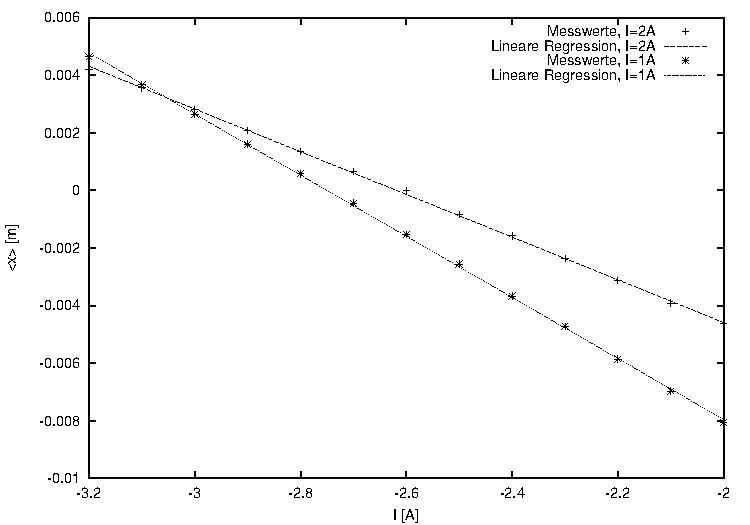
\includegraphics[width=1\textwidth]{./xbeamalignment.pdf}
	\caption{Messung des $x$-Versatzes des Strahls auf Schirm 3 in Abh�ngigkeit
 			des Stroms $I_\text{Q1MATCH}$ des horizontalen Dipols bei zwei
			verschiedenen Quadrupolstr�men $I_\text{V46MATCH}$
			(vgl. Tabelle \ref{tab:xbeamalign}).
			(2A)-Regressionsgerade gegeben durch
			$\frac{\langle x\rangle}{m}
				= -0,00741\cdot \frac{I}{\text{A}} - 0,01941$,
			(1A)-Regressionsgerade gegeben durch
			$\frac{\langle x\rangle}{m} 
				= -0,01061\cdot \frac{I}{\text{A}} - 0,02918$.}
			\label{fig:xbeamalign}
\end{figure}

\begin{figure}[ht]
    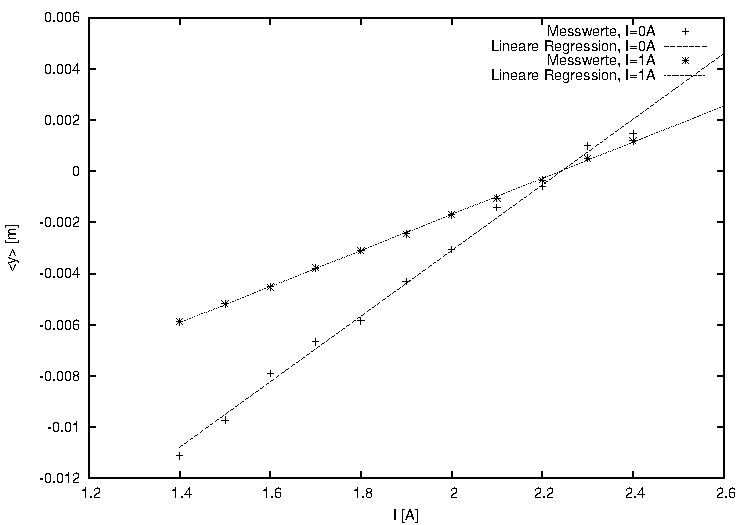
\includegraphics[width=1\textwidth]{./ybeamalignment.pdf}
	\caption{Messung des $y$-Versatzes des Strahls auf Schirm 3 in Abh�ngigkeit
 			des Stroms $I_\text{H15MATCH}$ des vertikalen Dipols bei zwei
			verschiedenen Quadrupolstr�men $I_\text{V46MATCH}$
			(vgl. Tabelle \ref{tab:ybeamalign}).
			(0A)-Regressionsgerade gegeben durch
			$\frac{\langle y\rangle}{m}
				= 0,0128 \cdot \frac{I}{\text{A}} - 0,0287$,
			(1A)-Regressionsgerade gegeben durch
			$\frac{\langle y\rangle}{m}
				 = 0,00704 \cdot \frac{I}{\text{A}} - 0,01579$.}
			\label{fig:ybeamalign}
\end{figure}

\begin{table}[ht]
\centering
\begin{tabular}{| >{$}c<{$} >{$}c<{$} |}
\hline
I_\text{V46MATCH}{ [A]}	&	\langle x \rangle \text{ [mm]}	 \\ [0.2ex]
\hline\hline
1,0	&	3,232253	\\
0,8	&	3,183226	\\
0,6	&	3,175869	\\
0,4	&	3,127449	\\
0,2	&	3,165518	\\
0,0	&	3,147471	\\
\hline
\end{tabular}
\caption{$x$-Versatz auf Schirm 3 f�r verschiedene Quadrupolstr�me bei
			$I_\text{Q1MATCH} = -3,055 \text{ A}$.}
	\label{tab:xbeamaligncheck}
\end{table}